\documentclass[crop,tikz]{standalone}
\usetikzlibrary{backgrounds}
\colorlet{blue}{cyan}
\tikzset{
  inverted/.style = {
    color=white,
    background rectangle/.style={fill},
    show background rectangle
  }
}
\usepackage{pgfplots}
\pgfplotsset{compat=1.18}

% Simple model for lightning conductor, see Arens, Chapter 32.2.
% The lines for constant potential w(t) = t + i y, y in Reals,
% and the field lines w(t) = x + i t, x in Reals are mapped as
% h^{-1}(w) = sqrt(w^2 - 1) to the shown plane.

\pgfplotsset{
  inverted/.style = {
    every axis legend/.append style={
      draw=white,
      fill=black,
      text=white
    }
  },
  every non boxed x axis/.append style={
    axis line style={-latex}
  },
  every non boxed y axis/.append style={
    axis line style={-latex}
  }
}

\begin{document}
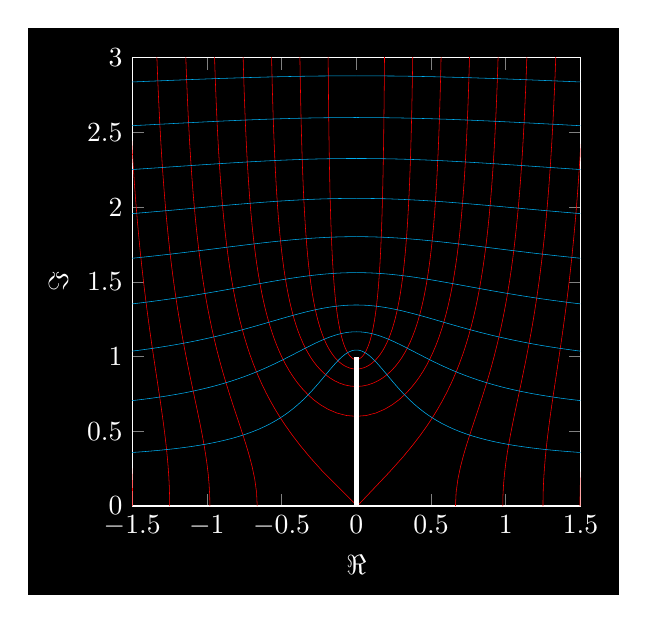
\begin{tikzpicture}[inverted,inverted]
  \pgfmathsetmacro{\numberoffieldlines}{10};
  \pgfmathsetmacro{\numberofpotentiallines}{10};
  \pgfmathsetmacro{\remin}{-2};
  \pgfmathsetmacro{\remax}{2};
  \pgfmathsetmacro{\immin}{0};
  \pgfmathsetmacro{\immax}{3};
  \begin{axis}[inverted,
    axis equal image,
    xmin={-1.5}, xmax={1.5},
    ymin={\immin}, ymax={\immax},
    xtick distance=0.5,
    ytick distance=0.5,
    xlabel={$\Re$},
    ylabel={$\Im$},
    samples=60,
    declare function = {
      absolute(\x,\y) = (((\x - \y)*(\x + \y) - 1)^2 + (2*\x*\y)^2)^(1/4);
      arctan(\x,\y) = atan2(2*\x*\y, (\x - \y)*(\x + \y) - 1);
      argument(\x,\y,\sx) = \x == 1 && \y == 0 ? pi/2 : ((\x < 0 && \y == 0) || (\x == 0 && \y > 0) ? -\sx*arctan(\x,\y) : arctan(\x,\y);
      % \sr is the sign of the root
      % \sx is the sign of x
      rez(\x,\y,\sr,\sx) = \sr*absolute(\x,\y)*cos(argument(\x,\y,\sx)/2);
      imz(\x,\y,\sr,\sx) = \sr*absolute(\x,\y)*sin(argument(\x,\y,\sx)/2);
    },
    ]
    % field lines
    \pgfplotsinvokeforeach{{\remax/\numberoffieldlines},{2*\remax/\numberoffieldlines},...,{\remax}}{
      \addplot[red,very thin,domain={\immin}:{\immax}] ({rez(#1,x,1,1)},{imz(#1,x,1,1)});
      \addplot[red,very thin,domain={\immin}:{\immax}] ({rez(-#1,x,-1,1)},{imz(-#1,x,-1,1)});
    }
    % lines of constant potential
    \pgfplotsinvokeforeach{{\immin + (\immax - \immin)/\numberofpotentiallines},{\immin + 2*(\immax - \immin)/\numberofpotentiallines},...,{\immax}}{
      \addplot[blue,very thin,domain={0}:{\remax}] ({rez(x,#1,1,-1)},{imz(x,#1,1,-1)});
      \addplot[blue,very thin,domain={\remin}:{0}] ({rez(x,#1,-1,1)},{imz(x,#1,-1,1)});
    }
    % lightning conductor
    \addplot[domain=0:1,ultra thick] (0,x);
  \end{axis}
\end{tikzpicture}
\end{document}
